\section{637 --- Average of Levels in Binary Tree}
Given a non-empty binary tree, return the average value of the nodes on each level in the form of an array.

\paragraph{Example 1:}

\begin{flushleft}

\textbf{Input}:

\begin{figure}[H]
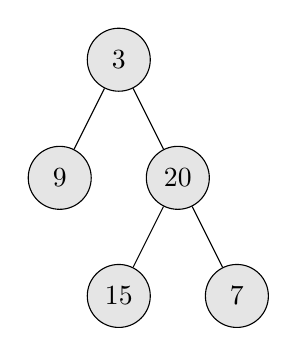
\begin{tikzpicture}
[every node/.style={draw, circle, fill=gray!20!, minimum size=8mm}]
\node{3}
child{node{9}}
child{node{20} child{node{15}} child{node{7}}};
\end{tikzpicture}
\end{figure}
\textbf{Output}: $[3, 14.5, 11]$

\textbf{Explanation}:

The average value of nodes on level 0 is 3,  on level 1 is 14.5, and on level 2 is 11. Hence return $[3, 14.5, 11]$.
\end{flushleft}

\paragraph{Note:}
\begin{itemize}
\item The range of node's value is in the range of 32-bit signed integer.
\end{itemize}

\subsection{BFS}
This is an easy question: just making use of breath first search with queue. 